\chapter{Experimental results with spatio-angular microscope}
\label{sec:results}
\begin{summary}
Akzeptanzwinkel

Bleaching

Strukturierte Beleuchtung
Berechnung zu wenige beads

sample mit dichter 3d verteilung von beads
\end{summary}

As one of the first attempts to use the spatio-angular illumination
system, I devised an experiment to determine the acceptance angle of a
microscope objective as a function of the embedding medium.

\begin{figure}[htbp]
  \centering
  \svginput{1}{tirf-exp}
  \caption{A fluorescent plane on a slide is embedded in oil, water or
    air. The thickness of the embedding medium is approximately
    $\unit[5]{\mu m}$. The focal plane SLM illuminates a disk with $\unit[30]{\mu
      m}$ diameter while a $15\times 15$ window is scanned over the
    MMA. The window corresponds to a square with $\unit[210]{\mu m}$
    on the side as opposed to \unit[3.6]{mm} BFP diameter {\bf right top:} 
    Typical camera image, the orange circle indicates the $\unit[30]{\mu
      m}$ illuminated area.
% 200 px diameter on LCoS
% 15x15 px full diameter is D=2*(R=f*NA) f=164.5/63=2.61  NA=1.38
% D=3.6mm -> D/256*15 = 210 um
    camera image.}
  \label{fig:tirf-exp}
\end{figure}



For the measurement a thin layer of fluorophores was applied with a
marker pen on three microscope slides. Furthermore, as a spacer, a
surrounding circle was painted with nail polish. After drying a drop
of immersion oil ($n=1.52$) or water ($n=1.33$) was added to two
samples. Then coverslips were added to all samples and sealed with
nail polish.

During the measurement the focal plane SLM projected a disk with
$\unit[30]{\mu m}$ diameter on the fluorescent plane. The illumination
angle was varied by stepping a window of $15\times 15$ pixels
(equivalent to 1/17th of the pupil diameter) over the pupil plane SLM.

For each angle, the sum of all the light on the camera is
recorded. The data is depicted in the three images in
\figref{fig:tirf-exp}. 

These images contain a bright disk whose diameter is growing with the
index of the embedding medium. The center of the disk corresponds to
the center of the pupil --- the optical axis of the microscope. Points
in the interior of the circle have an almost constant intensity
(residual fluctuations can be attributed to non-uniformity of the
illumination of the pupil plane SLM). For oil immersion the diameter
of the disk corresponds to the diameter of the pupil. As you can see
the pupil plane SLM was not centered perfectly on the optical axis in
this experiment.

If the index of the embedding medium is less than the index of the
immersion medium, then total internal reflection occurs on the
interface between coverslip and embedding medium for high incidence
angles. The excitation light can then no longer reach the
sample. Therefore, the disks in the plots for water and air are smaller.

FIXME winkel ausrechnen











gel with fluorophore \cite{Ruckerl}
\begin{figure}[!hbtp]
  \centering
  \svginput{1}{overview-bleach}
  \caption{The confocal measurements and images were kindly provided
    by Florian R\"uckerl (Institut Pasteur).}
  \label{fig:overview-bleach}
\end{figure}

\comment{
\jpginput{}{m_wf}{}
}

\begin{figure}[hbtp]
  \centering
  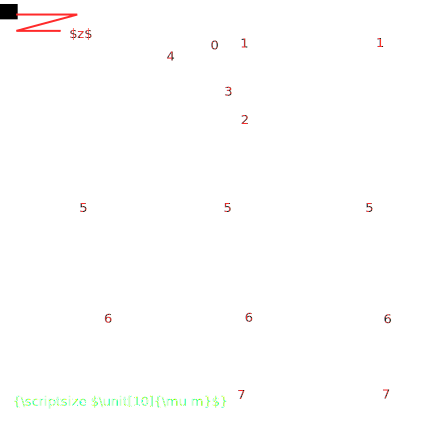
\includegraphics[width=12cm]{m_wf}
  \caption{Wide field stack of a three-dimensional distribution of
    yellow-green beads in agar. Sampling in $z$ is $\unit[1]{\mu m}$.}
  \label{fig:m_wf}
\end{figure}


\begin{figure}[hbtp]
  \centering
  \svginput{1}{m_sec}
  \caption{Computationally sectioned images. Note that two beads (4
    and 7) are very close to the border of the field of view and not
    fully illuminated.}
  \label{fig:m_sec}
\end{figure}


\begin{figure}[hbtp]
  \centering
  \svginput{1}{angular-beads}
  \caption{Spatio-angular controlled illumination of the beads from
    \figref{fig:m_sec}. The top left image shows bead number zero and
    so forth, the second image in the top shows bead number one and so
    on. The LCoS selectively illuminates the target bead and the MMA
    displays the pattern shown in \figref{fig:m_bfp_co}.}
  \label{fig:m_ang}
\end{figure}


\begin{figure}[!hbt]
  \centering
  \svginput{1}{montage-ang}
  \caption{}
  \label{fig:montage-ang}
\end{figure}




%%% Local Variables: 
%%% mode: latex
%%% TeX-master: "kielhorn_memi"
%%% End: 
